\section{Configurazione}
In questa sezione vengono trattati in primo luogo i requisiti minimi necessari per l'utilizzo dell'applicazione \textit{HDViz} e successivamente come poter installare il prodotto in locale direttamente dal \glo{repository} pubblico \glo{GitHub} del gruppo \Gruppo{}.  
\subsection{Requisiti di sistema}
Per far si che le operazioni di installazione e avvio del prodotto avvengano correttamente e che si possa aver accesso a tutte le funzionalità, è necessario avere nella propria macchina i seguenti software.
{
\setlength\arrayrulewidth{0.95pt}
\renewcommand{\arraystretch}{1.5}
\begin{longtable}{C{3cm} | C{3cm} | C{9cm}}
\rowcolor{coloreRosso}

\textcolor{white}{\textbf{Software}}&
\textcolor{white}{\textbf{Versione}}&
\textcolor{white}{\textbf{Riferimento per il downlaod}} \\
\endfirsthead
\rowcolor{white}\multicolumn{3}{C{15cm}}{\textit{Continua nella pagina successiva...}}\\
\endfoot
\rowcolor{white}\caption{Requisiti di sistema}
\endlastfoot
	
	\textbf{Node.js} &
	14.16.x &
	\textcolor{blue}{\url{https://nodejs.org/it/}} \\
 
	\textbf{Npm} & 
	7.x &
	Integrato nel download di Node.js \\
	
	\textbf{PostgreSQL} &
	13.x &
	\textcolor{blue}{\url{https://www.postgresql.org/download/}} \\
\end{longtable}	

}
\subsection{Requisiti hardware}
Per avere delle prestazioni accettabili dell'applicazione è preferibile avere almeno i seguenti componenti hardware.
{
\setlength\arrayrulewidth{0.95pt}
\renewcommand{\arraystretch}{1.5}
\begin{longtable}{C{4cm} | C{4cm}}
\rowcolor{coloreRosso}

\textcolor{white}{\textbf{Componente}}&
\textcolor{white}{\textbf{Requisito}} \\
\endfirsthead
\endfoot
\rowcolor{white}\caption{Requisiti hardware}
\endlastfoot
	
	\textbf{Processore} &
	 Quad-Core 3,2 GHz \\
 
	\textbf{RAM} & 
	8GB DDR4 \\

\end{longtable}	
}

\newpage

La connessione internet ideale dovrebbe essere di almeno 80Mb/s in download per assicurare i seguenti tempi di risposta (in secondi) della web app. 
{
\setlength\arrayrulewidth{0.95pt}
\renewcommand{\arraystretch}{1.5}
\begin{longtable}{C{2cm} | C{10cm}}
\rowcolor{coloreRosso}

\textcolor{white}{\textbf{Tempo}}&
\textcolor{white}{\textbf{Operazione}} \\
\endfirsthead
\endfoot
\rowcolor{white}\caption{Prestazioni ottimali}
\endlastfoot
	
	\textbf{2} &
	Caricamento di un dataset di 2Mb;  \\
 
	\textbf{7} & 
	Applicazione di un algoritmo  di riduzione dimensionale con 4 dimensioni e 500 punti in totale; \\
	
	\textbf{2} &
	Visualizzazione di un grafico con 500 punti.  \\	
	
\end{longtable}	
}

\subsection{Browser}
L'applicazione è stata testata e quindi resa compatibile con le ultime versioni dei browser maggiormente utilizzati al momento.
{
\setlength\arrayrulewidth{0.95pt}
\renewcommand{\arraystretch}{1.5}
\begin{longtable}{C{4cm} | C{4cm}}
\rowcolor{coloreRosso}

\textcolor{white}{\textbf{Browser}}&
\textcolor{white}{\textbf{Versione}} \\
\endfirsthead
\endfoot
\rowcolor{white}\caption{Browser e versioni compatibili}
\endlastfoot
	
	\textbf{Chrome} &
	 87 \\
 
	\textbf{Edge} & 
	79\\
	
	\textbf{Mozilla Firefox} &
	 84 \\
 
	\textbf{Safari} & 
	13.1 \\
	
\end{longtable}	
}

\newpage

\section{Installazione}
Per utilizzare l'applicazione web è necessario:
\begin{itemize}
\item Clonare la repository (\textbf{Obbligatorio})
\item Importare il database (\textit{Opzionale})
\item Avviare il server (\textit{Opzionale})
\item Avviare la web app (\textbf{Obbligatorio})
\end{itemize}
\subsection{Clonare la repository}
\begin{enumerate}
	\item Scaricare il codice come file .zip direttamente dal repository CodeBusters-HDViz:
		\begin{center}
			\textcolor{blue}{\url{https://github.com/CodeBusterswe/CodeBusters-HDviz}}
		\end{center}	
	Oppure, con \glo{Git} installato in locale, è possibile clonare il repository con il comando:
		\begin{center}
			\textcolor{coloreRosso}{\textbf{git clone https://github.com/CodeBusterswe/CodeBusters-HDviz}}
		\end{center}
      
	\item Localizzare da terminale la cartella in cui si è stato estratto/clonato il prodotto:  
		\begin{center}
			\textcolor{darkgray}{\textbf{cd percorso\textbackslash CodeBusters-HDViz}}
 		\end{center}
\end{enumerate}
\subsection{Importare il database}
\begin{enumerate}
\item Installare PostegreSQL e pgAdmin dal sito :
	\begin{center}
			\textcolor{blue}{\url{https://www.postgresql.org/download/}}
	\end{center}	
\item Creare un nuovo database
\item Fare il restore del database utilizzando il file "dumbDB" presente in "./server"
\end{enumerate}
\subsection{Avviare il server}
\begin{enumerate}
\item Entrare nella cartella "server"
	\begin{center}
			\textcolor{coloreRosso}{\textbf{cd server}}
 	\end{center}
\item Nel caso di primo avvio, digitare:
	\begin{center}
			\textcolor{coloreRosso}{\textbf{npm install}}
 	\end{center}

\newpage 	
 	
\item Controllare che i valori impostati nel file "./config/default.js" corrispondano a quelli impostati in postegreSQL:
\begin{itemize}
\item 'USER\underline{}NAME' : nome utente dell'account;
\item 'PASSWORD' : password dell'account;
\item 'HOST' : porta di postegreSQL;
\item 'DB\_NAME' :  nome del db precedentemente creato;
\end{itemize}
\item Avviare il server con il comando:
	\begin{center}
			\textcolor{coloreRosso}{\textbf{npm start}}
 	\end{center}
\end{enumerate}
\subsection{Avviare la web app}
\begin{enumerate}
\item Entrare nella cartella "client"
	\begin{center}
			\textcolor{coloreRosso}{\textbf{cd client}}
 	\end{center}
\item Nel caso di primo avvio digitare il comando:
		\begin{center}
			\textcolor{coloreRosso}{\textbf{npm install}}
 		\end{center}
\item Fare la build dell'app con il comando:
		\begin{center}
			\textcolor{coloreRosso}{\textbf{npm run build}}
 		\end{center}
\item Nel caso di primo avvio dell’applicazione sul sistema, digitare:
		\begin{center}
			\textcolor{coloreRosso}{\textbf{npm install -g serve}}
 		\end{center}	     
\item Digitare poi:
		\begin{center}
			\textcolor{coloreRosso}{\textbf{serve -s build -l 4000}}
 		\end{center}		
\end{enumerate}

L'applicazione sarà disponibile aprendo l'indirizzo fornito dal terminale.

\begin{figure}[H]
		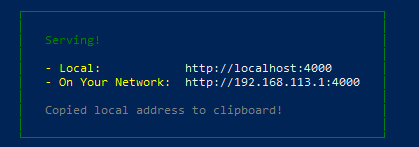
\includegraphics[scale=1]{Images/install.png}
		\centering
		\caption{Avvio dell'applicazione}
\end{figure}
  			